\textbf{See the instruction for questions \inteval{\value{question}+1} to \inteval{\value{question}+2}.}

\begin{figure}[H]
    \centering
    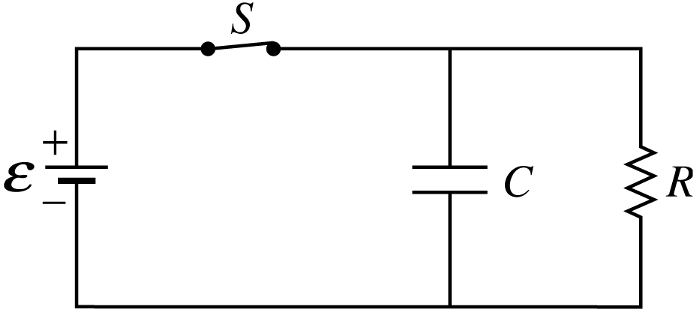
\includegraphics[scale=0.3]{images/img-004-004.png}
\end{figure}

Switch $S$ in the circuit shown above has been closed for a long time.

% Multiple Choice Question 7
\begin{questions}\setcounter{question}{6}\question
Which of the following is the correct expression for the current in the resistor?

\begin{oneparchoices}
\choice $\dfrac{\mathcal{E}}{R}$
\choice $\dfrac{C \mathcal{E}}{R}$
\choice $C \mathcal{E}$
\choice $\dfrac{\mathcal{E}}{R C}$
\choice Zero
\end{oneparchoices}\end{questions}

% Multiple Choice Question 8
\begin{questions}\setcounter{question}{7}\question
Suppose that the switch is opened at time $t=0$. Which of the following combinations of a differential equation and an initial condition can be used to solve for the charge $Q(t)$ on the upper plate of the capacitor as a function of time $t$?

\tabto{0.75cm} \underline{Differential Equation}
\tabto{6.00cm} \underline{Initial Condition}

\begin{choices}
\choice $\dfrac{Q}{C}-R \dfrac{\diff Q}{\diff t}=0$           \tabto{5.25cm} $Q(0)=C \mathcal{E}$
\choice $\dfrac{Q}{C}-R \dfrac{\diff Q}{\diff t}=\mathcal{E}$ \tabto{5.25cm} $Q(0)=0$
\choice $\dfrac{Q}{C}+R \dfrac{\diff Q}{\diff t}=\mathcal{E}$ \tabto{5.25cm} $Q(0)=C \mathcal{E} $
\choice $\dfrac{Q}{C}+R \dfrac{\diff Q}{\diff t}=0$           \tabto{5.25cm} $Q(0)=0$
\choice $\dfrac{Q}{C}+R \dfrac{\diff Q}{\diff t}=0$           \tabto{5.25cm} $Q(0)=C \mathcal{E}$
\end{choices}\end{questions}
